\subsection{Time Series}

To analyze time series data we use three models to predict the trajectory of the number of accidents with deaths.
We split the series into ‘Train’ and ‘Test’ putting off the last year for testing.
For time series analysis we fit ARIMA model [ SARIMAX(0, 1, 1)(1, 0, 1, 12) ] with its AutoARIMA implementation,
TBATS with Box-Cox transformations and year seasonality and Prophet with additive seasonality,
linear growth and MCMC samples using their implementation in $\verb|sktime|$.
In order to measure the error of prediction we use MAPE (Mean average percentage error).
The choice of the metric can be attributed to the need to measure not the absolute value of the error, but the normed one,
as these results can be interpreted better. The results of the models are shown in the table. \\

\begin{table}[htpb]
	\centering
	\label{tab:mape}
	\begin{tabular}{|c|c|}
		\hline
		& MAPE \\
		\hline
		ARIMA & $0.2697$ \\
		TBATS	& $0.2951$ \\
		\textbf{Prophet}	& $0.2271$ \\ 
		\hline
	\end{tabular}
	\caption{\textbf{Mean Average Percentage Error}}
\end{table}
\noindent
We visualize the predictions of each model. As it turns out the best model is Prophet with MAPE equal to 0.2271.
\subsection{Imbalanced Classification}
In this part we carefully examine the approach to imbalanced classification used in this research.
In order to measure the accuracy of prediction we choose Cohen-Kappa coefficient and Matthews Correlation Coefficient.
We also use AUC-Pr to measure the quality of the model. The reason we choose these metrics instead of usual accuracy is precisely the imbalance we have.
In that case usual accuracy happens to be skewed towards majority class and does not accurately measure the quality of the result.
Moreover, we separately measure precision and recall of two classes as well.
First of all we focus our attention on classical methods and use logistic regression and boosting methods.
As hyperparameters we select class weights, significantly downsizing the majority class the results of two methods are shown on the graph
\ref{fig:ts_predictions}.

\begin{figure}[htpb!]
	\centering
	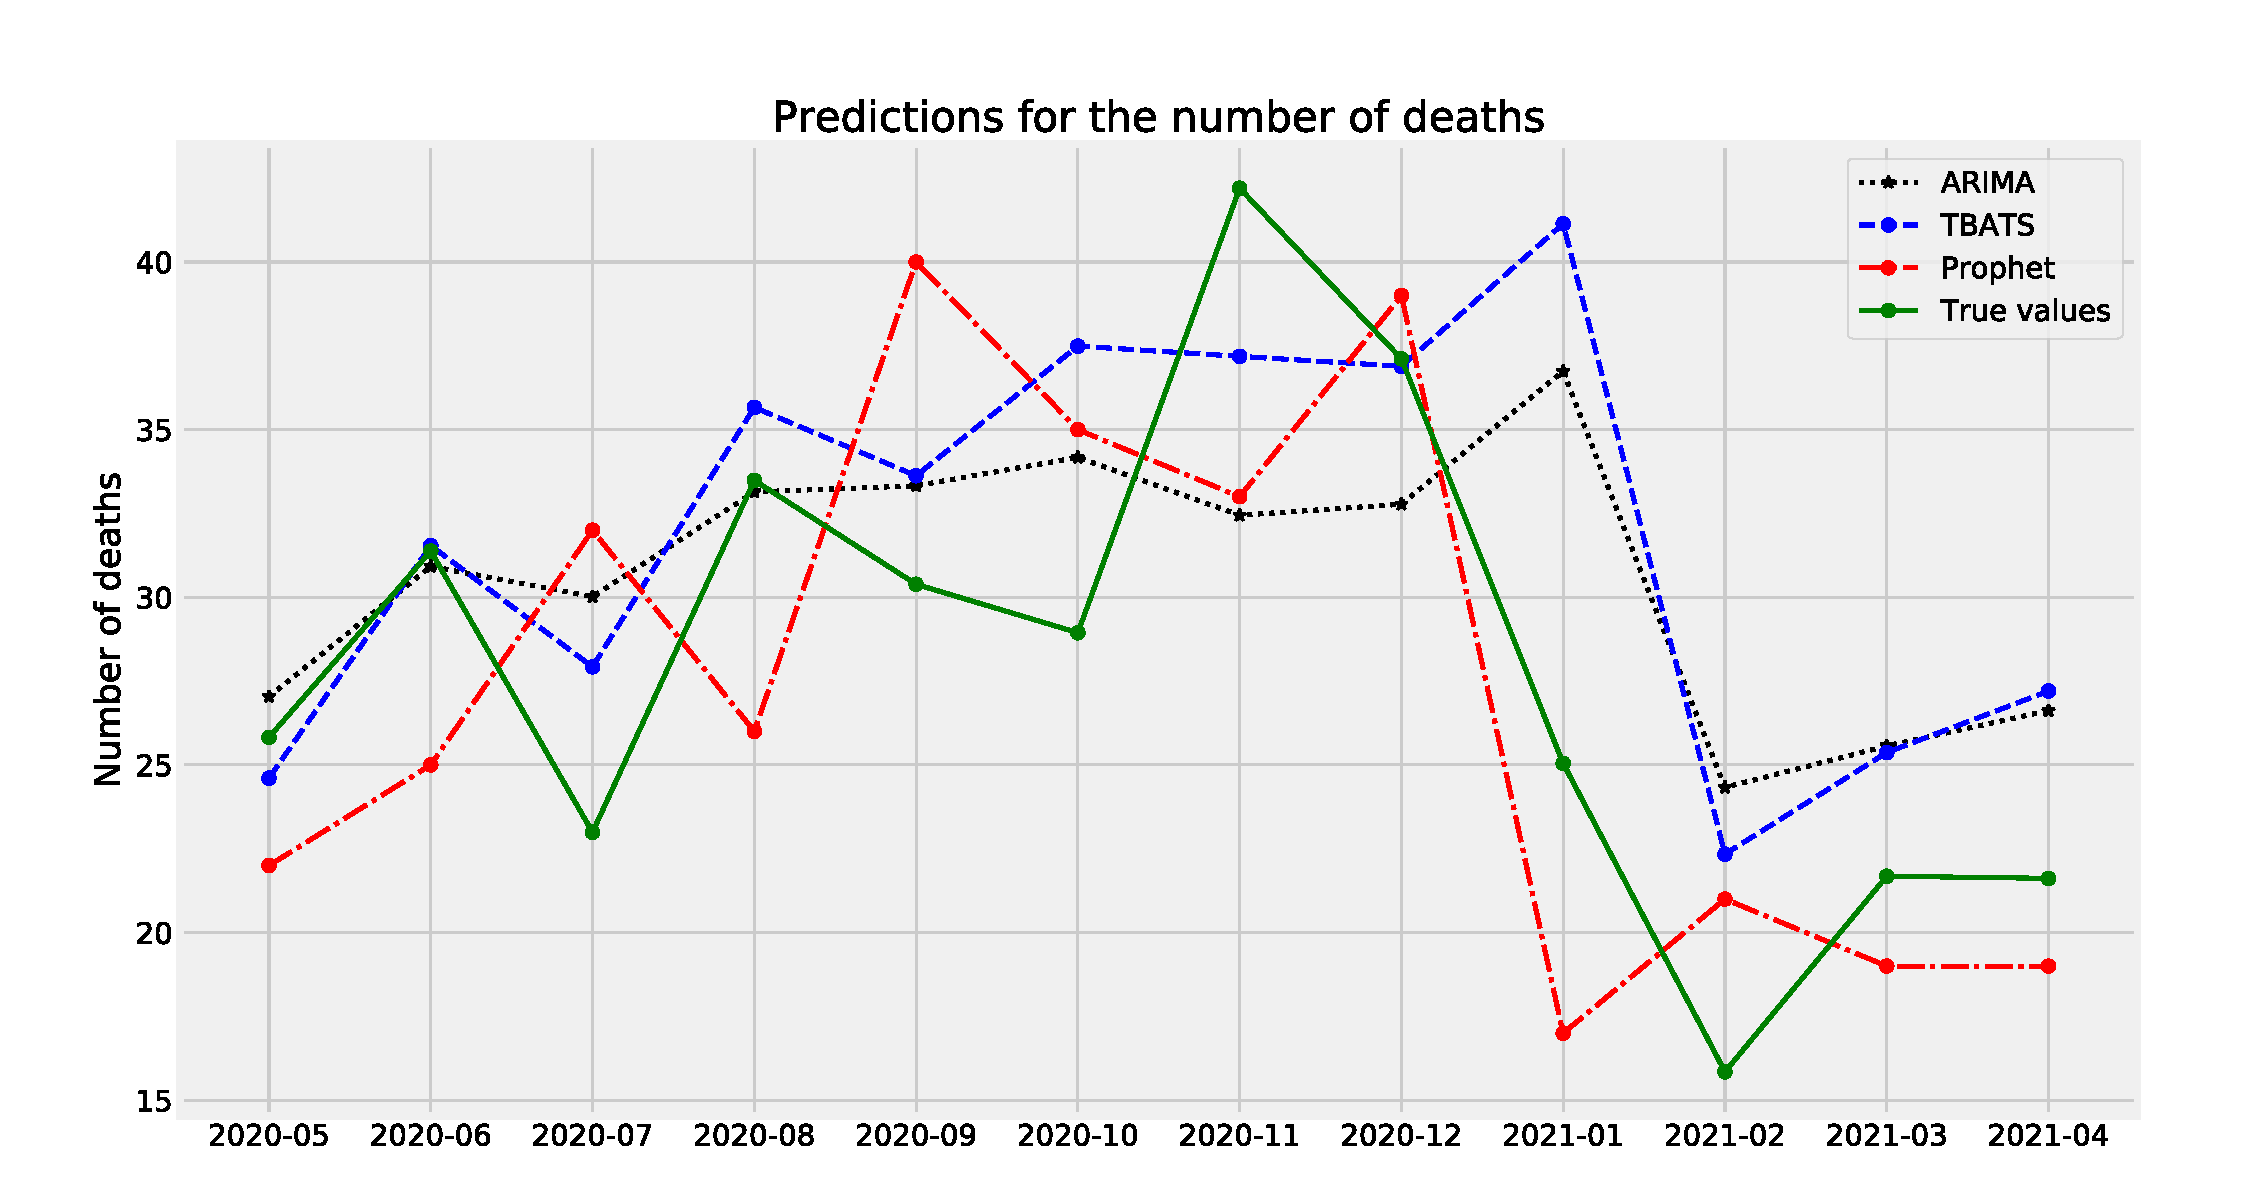
\includegraphics[width=0.8\textwidth]{../imgs/pdf_files/ts_predictions.pdf}
	\caption{\textbf{Time Series Death Predictions}}
	\label{fig:ts_predictions}
\end{figure}
\noindent
In order to meaningfully estimate the results of the two models we look at probabilities the models assign to each class
for every object and then compute metrics multiple times while changing the binarization threshold.
We can see that two models give comparable results with boosting performing slightly better. The results can be interpreted as follows.
As it was stated before two classes are heavily imbalanced, and they do overlap as well.
That highly influences precision of a minority class. It is very low.
The only pick of precision occurring while the threshold is low is attributed to the tiny sample of minority class objects
that the models are quite sure about, however this result cannot be interpreted as successful one due to recall being very low in this case. 
Low precision of minority class consequently influences metrics for imbalanced classification that we use. 
It is clear from the graphs, that both models are unable to give meaningful accuracy.
As authors think, it happens largely to the overlap of data.
That means that existing predictors are insufficient to accurately separate to classes.
Meaning that we actually really don’t have other valuable features, that may help us to predict the severity better. \\
In attempt to tackle that problem we fit models, specifically designed for imbalanced datasets.
Their results can be seen in the table.

\begin{table}[htpb]
	\centering
	\label{tab:metircs_imb}
	\resizebox{15cm}{!}
	{
\begin{tabular}{|c|c|c|c|c|c|c|c|}
	\hline
	 & \textbf{Cohen-Kappa} &	\textbf{MCC} & \textbf{AUC-Pr} & \textbf{Precision(Majority)} & \textbf{Precision(Minority)} & \textbf{Recall(Majority)} &	
 \textbf{Recall(Minority)} \\
	 \hline
		One-Class SVM & -0.025	& -0.05	& 0.044	& 0.938 &	0.036	& 0.491	& 0.371 \\
		\hline
		Isolation Forest & \textbf{0.054} & \textbf{0.054} &	\textbf{0.054}	& \textbf{0.954} &	\textbf{0.094}	& \textbf{0.039}	& 0.122 \\
		\hline
		Local Outlier Factor & 0.001 & 0.005 & \textbf{0.054} & 0.953 & 0.050	& 0.314	& \textbf{0.696} \\
		\hline
	\end{tabular}
}
\caption{\textbf{Imbalanced Classification Metrics}}
\end{table}
\noindent
As we can see these methods perform worse, with Isolation Forest giving slightly better results.
The reason for that may be the overlap as well.
And given the fact that all the methods are based on either drawing a hyperplane in object space or counting the distance
they cannot discriminate objects of two classes as those objects are very close to each other.
